\documentclass[11pt]{article}

\usepackage[margin=1in]{geometry}
\usepackage[T1]{fontenc}
\usepackage[utf8]{inputenc}
\usepackage{lmodern}
\usepackage{setspace}
\usepackage{lineno}
\usepackage{amsmath,amssymb}
\usepackage{graphicx}
\usepackage{booktabs}
\usepackage{siunitx}
\usepackage{xcolor}
\usepackage{multirow}
\usepackage{array}
\usepackage[numbers,sort&compress]{natbib}
\usepackage[colorlinks=true,allcolors=blue]{hyperref}

\graphicspath{{figures/}}

\title{Skill-Augmented Frontier Agents Nearly Saturate\\
BixBench-Verified-50}
\author{Xiaoyu Zhang\textsuperscript{1,*}}
\date{}

\begin{document}

\maketitle

\begin{center}
\textsuperscript{1}California State University San Marcos, San Marcos, CA, USA\\
\textsuperscript{*}Correspondence: \texttt{xiaoyu@csusm.edu}
\end{center}

\begin{abstract}
\noindent
Large language model (LLM) agents are increasingly used for biological data
analysis, but prior benchmark results have given a mixed picture of whether
they are ready for routine bioinformatics work. The original BixBench study
reported only $\sim$17--21\% accuracy for frontier agents on open-answer
bioinformatics questions \citep{mitchener2025bixbench}. Subsequent curation
of BixBench-Verified-50 removed or revised ambiguous items, revealing much
higher performance for modern agents \citep{phylo2026}. Here we evaluate
three frontier-model configurations on the 50 verified questions using the
same local benchmark, prompt structure, answer format, and grading pipeline:
GPT-5.4 with Claude Scientific Skills and no web access, Claude Opus~4.7 with
Claude Scientific Skills and no web access, and GPT-5.5 with Claude
Scientific Skills, bioSkills, and web access. The three configurations
achieve 88.0\% (44/50), 84.0\% (42/50), and 98.0\% (49/50) accuracy,
respectively. The remaining GPT-5.5 error is not a clear analytical failure:
the agent correctly computed Spearman correlations on the distributed
\texttt{CRISPRGeneEffect.csv} values and selected CCND1, whereas the
reference answer is recovered only after interpreting stronger essentiality
as the opposite sign of the raw gene-effect score. Offline errors mainly
occurred when agents lacked pathway, organism-annotation, BUSCO, or
PhyKIT-related resources. These results show that frontier agents equipped
with high-quality scientific skills can nearly saturate a curated
bioinformatics benchmark, while also emphasizing that question wording, score
sign conventions, and access to current external resources remain decisive
for reliable evaluation.
\end{abstract}

\doublespacing
\linenumbers

\section{Introduction}

The last 18 months have seen an explosion of LLM-based agents targeted at
biological research, ranging from general-purpose co-scientists such as
Biomni \citep{huang2025biomni} and K-Dense \citep{li2025kdense} to
multi-agent frameworks such as BioAgents \citep{mehandru2025bioagents}.
Bioinformatics is a natural domain for these systems: it is dominated by
short, well-specified analytical tasks (e.g.\ ``run DESeq2 with these
covariates'') that combine code, statistics, and biological judgement. At
the same time, even small mistakes in normalization, filtering, or library
choice can change scientific conclusions. Whether agents are good enough
for this work, and what configuration of components actually drives
accuracy, are open questions.

The first systematic attempt to measure agent performance on real
bioinformatics workflows was BixBench \citep{mitchener2025bixbench}, a
benchmark of nearly 300 multiple-choice and open-answer questions derived
from 53 published Jupyter analysis notebooks (``capsules''). The original
report concluded that frontier models in early 2025 were not yet ready:
even the best agent achieved only $\sim$17--21\% open-answer accuracy and
no better than random performance in the multiple-choice setting. A
subsequent curation effort by Phylo produced BixBench-Verified-50, a
50-question subset across 33 capsules in which problematic questions were
removed, wording was clarified, and expected answers were corrected where
domain experts judged the original ground truth unreliable
\citep{phylo2026,hfbixverified}. After this cleanup, reported accuracy
rose sharply: Biomni Lab reached 88.7\%, K-Dense Web reached 90.0\%, and
SciAgent-Skills reported 92.0\% with Claude Opus 4.6
\citep{phylo2026,kdense2026,sciagent2026}. The size of this shift raises
an important question for evaluation: are modern biology agents genuinely
becoming competent, or are scores mainly improving because the benchmark
is now less noisy?

In parallel, open-source ``skill libraries'' have appeared that give
agents bioinformatics-aware code patterns, package conventions, database
usage notes, and troubleshooting guidance. Claude Scientific Skills
(subsequently broadened as Scientific Agent Skills) provides more than 120
scientific skills across bioinformatics, cheminformatics, statistics, and
scientific writing \citep{kdenseskills,kdensescientificagentskills}.
bioSkills provides SKILLS.md files focused specifically on bioinformatics
workflows for coding agents such as Claude Code, Codex, Gemini, and related
tools \citep{bioskills}. These libraries follow the Agent Skills pattern in
which each skill is a version-controlled markdown file that the host agent
loads when relevant \citep{anthropicskills}. This format is important for
scientific work because it makes procedural knowledge inspectable by domain
experts rather than hiding it inside model weights.

This work evaluates that question directly by running three contemporary
agent configurations on BixBench-Verified-50 with identical scaffolding
and scoring (Section~\ref{sec:methods}). The configurations vary the base
model, skill-library coverage, and web access. We report overall accuracy,
per-capsule and per-category breakdowns, agent-vs-agent agreement, and a
qualitative analysis of every residual error. The main result is simple:
skill-augmented frontier agents now nearly saturate this curated
bioinformatics benchmark. Even the offline configurations reach 84--88\%,
while the GPT-5.5 configuration with Claude Scientific Skills, bioSkills,
and web access reaches 98\% (49/50). The only remaining GPT-5.5 miss is
best understood as a sign-convention ambiguity in the essentiality score,
not as an incorrect statistical computation. We therefore conclude that
frontier agents equipped with curated scientific skills are already
competitive on short, well-specified BixBench-style bioinformatics
questions, while longer, open-answer, and trace-scored evaluations remain
necessary before these systems can be considered ready for unsupervised
research.

\section{Related Work}

\paragraph{Bioinformatics benchmarks for agents.}
BixBench \citep{mitchener2025bixbench} introduced a 53-capsule, $\sim$300-question
benchmark of practical bioinformatics tasks drawn from peer-reviewed
notebooks, scored either by exact-match MCQ or LLM-judged open answer.
The Phylo BixBench-Verified-50 subset \citep{phylo2026} kept 50 of those
questions, revising or removing items where domain experts disagreed
with the original gold answer or context. Several earlier benchmarks
target adjacent skills: LAB-Bench \citep{laurent2024labbench} measures
literature recall, figure interpretation, database lookup, and sequence
manipulation as 8 separate capabilities; BioCoder \citep{tang2024biocoder}
measures bioinformatics-specific code generation against a fuzz-tested
suite; ScienceAgentBench \citep{chen2024scienceagent} measures end-to-end
data-science programs across four scientific disciplines including
bioinformatics; DSBench \citep{jing2024dsbench} and DataSciBench
\citep{zhang2025datasci} measure general data-science agent capability.
BixBench is distinguished from these by its explicit grounding in
published analytical workflows and its requirement that the agent
produce a numerically correct answer rather than runnable code.

\paragraph{Bioinformatics agents.}
Biomni \citep{huang2025biomni} is a generalist biomedical agent built on
a unified environment of 150 tools, 59 databases, and 106 software
packages, and has been applied to causal gene prioritization, drug
repurposing, and rare disease diagnosis. K-Dense Analyst
\citep{li2025kdense} is a hierarchical multi-agent system for
bioinformatics that uses planning + validated execution and reports a
59\% relative gain over its base model on the original BixBench (29.2\%
vs.\ 18.3\%). BioAgents \citep{mehandru2025bioagents} is a multi-agent
framework using small fine-tuned LLMs and retrieval-augmented generation
to assist with workflow construction. Specialized scientific-skill
libraries are emerging as a lighter-weight alternative: SciAgent-Skills
\citep{sciagent2026}, Claude Scientific Skills \citep{kdenseskills},
and bioSkills \citep{bioskills} package domain knowledge as markdown
files that any agent following Anthropic's open Agent Skills standard
\citep{anthropicskills} can load on demand. The rapid progression on
BixBench-Verified-50 --- from 65.3\% for vanilla Claude Code (Opus 4.6)
\citep{phylo2026} to 92.0\% for Claude Code with SciAgent-Skills
\citep{sciagent2026} --- suggests that skill libraries provide most of the
contribution of more elaborate agent architectures at a small fraction of
the engineering cost.

\section{Methods}\label{sec:methods}

\subsection{Dataset}
We evaluate on BixBench-Verified-50, a curated 50-question subset of
BixBench v1.5 spanning 32 distinct analytical capsules
\citep{phylo2026}.\footnote{Capsule \texttt{bix-16} appears with three
questions in our subset and the dataset description on Hugging Face
reports 33 capsules; the difference of one is consistent with our local
mapping of question UUIDs to capsule UUIDs.} Each question is
formulated as a multiple-choice question with four content options
(A--D in the dataset) plus a fixed ``Insufficient information to answer
the question'' refusal option (B in our prompt template), and is
accompanied by a capsule directory containing the input data files
referenced by the question. Reference notebooks were removed prior to
evaluation so that agents had to derive each answer from the data alone.

\subsection{Agent configurations}
We compare three contemporary frontier-model agent configurations
(Table~\ref{tab:configs}). All three use the same prompt template, the
same single-question-per-trajectory protocol, and identical answer-grading
logic. Each agent is given (i) the question text and answer options,
(ii) a path to the capsule directory, and (iii) a writable artifacts
directory where it may write code, intermediate files, and notes.

\begin{table}[ht]
\centering
\caption{Agent configurations evaluated. ``Skills'' columns indicate
whether the agent had access to the Claude Scientific Skills library
\citep{kdenseskills} or the bioSkills library \citep{bioskills}.}
\label{tab:configs}
\begin{tabular}{llccc}
\toprule
Label                  & Base model         & Claude Sci. Skills & bioSkills & Web \\
\midrule
GPT-5.4 (no web)       & GPT-5.4 (Codex)    & \checkmark         &           &     \\
Opus 4.7 (no web)      & Claude Opus 4.7    & \checkmark         &           &     \\
GPT-5.5 (web)          & GPT-5.5 (Codex)    & \checkmark         & \checkmark& \checkmark \\
\bottomrule
\end{tabular}
\end{table}

The Claude Scientific Skills library \citep{kdenseskills} provides more
than 120 SKILL.md files covering bioinformatics workflows including
BioPython, Scanpy, PyDESeq2, STAR, HISAT2, phylogenetics, and ADMET, plus
broader scientific skills for statistics, machine learning, literature
review, and writing. The bioSkills library \citep{bioskills} adds
bioinformatics-specific code patterns, best practices, and examples
ranging from sequence work to single-cell and population genetics. Both
libraries use markdown skill files with YAML frontmatter and prose that
the host agent loads on demand. In all three configurations the agent is
allowed to write and execute Python, R, and shell code in a sandboxed
environment.

\subsection{Prompt template}
Each agent received a prompt of the form (paths abbreviated for space):

\begin{quote}\small\ttfamily
Question: \textit{<text>}\\
Local paths: \\
\hspace*{1em}- Capsule data directory: \textit{<capsule\_dir>}\\
\hspace*{1em}- Writable artifacts directory: \textit{<artifacts\_dir>}\\
Requirements: Inspect the capsule data, form a plan, then write and
execute any code needed to answer the question as rigorously as
possible. \textit{[Web allowed/forbidden depending on configuration]}.
The reference notebook has been removed.\\
Answer options: (A) \dots (B) Insufficient information \dots (E) \dots
\end{quote}

The agent's final answer was a single option letter (A--E). When the
agent selected the refusal option (``Insufficient information''), the
response was treated as ``unsure'' for coverage statistics but counted
as incorrect for accuracy.

\subsection{Scoring}
Predicted letters were compared to expert-curated targets from
BixBench-Verified-50. The set of letter labels was independently shuffled
per agent at prompt time, so target letters differ across agents for the
same content question; this prevents any positional bias from inflating
agreement statistics. We report:
\begin{itemize}\itemsep0pt
\item \textbf{Accuracy} = $n_{\text{correct}}/50$, with Wilson 95\%
binomial confidence intervals.
\item \textbf{Coverage} = $n_{\text{sure}}/50$, the fraction of questions
where the agent did not invoke the refusal option.
\item \textbf{Precision} = $n_{\text{correct}}/n_{\text{sure}}$,
accuracy among questions the agent attempted.
\item \textbf{Per-capsule accuracy}: pooled across the 1--4 questions
per capsule.
\item \textbf{Pairwise agreement on correctness}: fraction of questions
on which two agents both succeed or both fail.
\end{itemize}

\subsection{Data and code availability}
Full per-question prediction CSVs (\texttt{combined.csv}), grading
JSONs (\texttt{combined\_graded.json}), and grading reports
(\texttt{combined\_grading\_report.md}) are provided in
\texttt{results/\{codex\_agent,claude\_code\_agent,codex\_agent\_5.5\}/}.
Analysis scripts (\texttt{agent\_results.py}, \texttt{make\_figures.py})
and the per-question correctness matrix
(\texttt{per\_question\_correctness.csv}) are provided alongside this
manuscript.

\section{Results}\label{sec:results}

\subsection{Overall accuracy}

Table~\ref{tab:overall} and Figure~\ref{fig:accuracy} summarize overall
performance. The two offline configurations achieve 84.0\% (Opus~4.7)
and 88.0\% (GPT-5.4); the web-enabled GPT-5.5 configuration achieves
98.0\%. Because each configuration was run once, we interpret the
differences as an observed benchmark comparison rather than a replicate
estimate of model variance. Coverage is high in all three configurations
(92--100\%); the agents rarely invoked the refusal option.

\begin{table}[ht]
\centering
\caption{Overall results on BixBench-Verified-50 ($n=50$).
$n_\text{correct}$: questions answered correctly; $n_\text{sure}$:
questions on which the agent did not return the refusal option;
Coverage~$=n_\text{sure}/n$; Precision~$=n_\text{correct}/n_\text{sure}$.
95\% CI is Wilson binomial.}
\label{tab:overall}
\begin{tabular}{lcccccc}
\toprule
Configuration       & Accuracy & 95\% CI         & $n_\text{correct}$/50 & Coverage & Precision \\
\midrule
GPT-5.4 (no web)    & 88.0\%   & [76.2, 94.4]    & 44                    & 94.0\%   & 93.6\% \\
Opus 4.7 (no web)   & 84.0\%   & [71.5, 91.7]    & 42                    & 92.0\%   & 91.3\% \\
GPT-5.5 (web)       & \textbf{98.0\%} & [89.5, 99.6] & \textbf{49}        & 100.0\%  & 98.0\% \\
\bottomrule
\end{tabular}
\end{table}

\begin{figure}[ht]
  \centering
  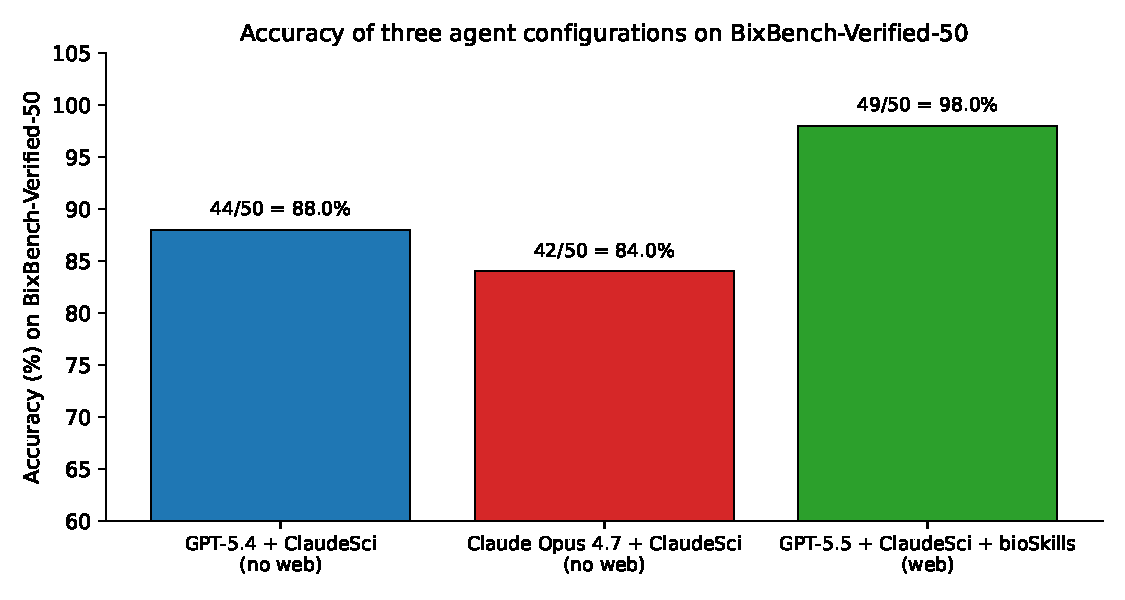
\includegraphics[width=0.78\linewidth]{fig1_accuracy.pdf}
  \caption{Accuracy of three frontier-model agent configurations on
  BixBench-Verified-50. Bars show one complete benchmark run per
  configuration; no run-level error bars are shown. GPT-5.5 with the
  bioSkills overlay and web access exceeds both offline configurations.}
  \label{fig:accuracy}
\end{figure}

\subsection{Comparison to published results}

Figure~\ref{fig:leaderboard} places these results in the context of
previously reported BixBench-Verified-50 numbers. Our weaker offline
configuration (Opus~4.7 + ClaudeSci, 84.0\%) substantially exceeds the
vanilla Claude Code (Opus~4.6) baseline reported by Phylo (65.3\%)
\citep{phylo2026}, although the model version and skill availability are
both different. Our GPT-5.4 (no web) configuration at 88.0\% is
comparable to Biomni Lab's reported 88.7\% and within the band of
K-Dense Web (90.0\%) and SciAgent-Skills (92.0\%). The GPT-5.5 (web)
configuration sets a new high water mark for BixBench-Verified-50 at
98.0\%, exceeding the previous best (92.0\%) by 6 percentage points.

\begin{figure}[ht]
  \centering
  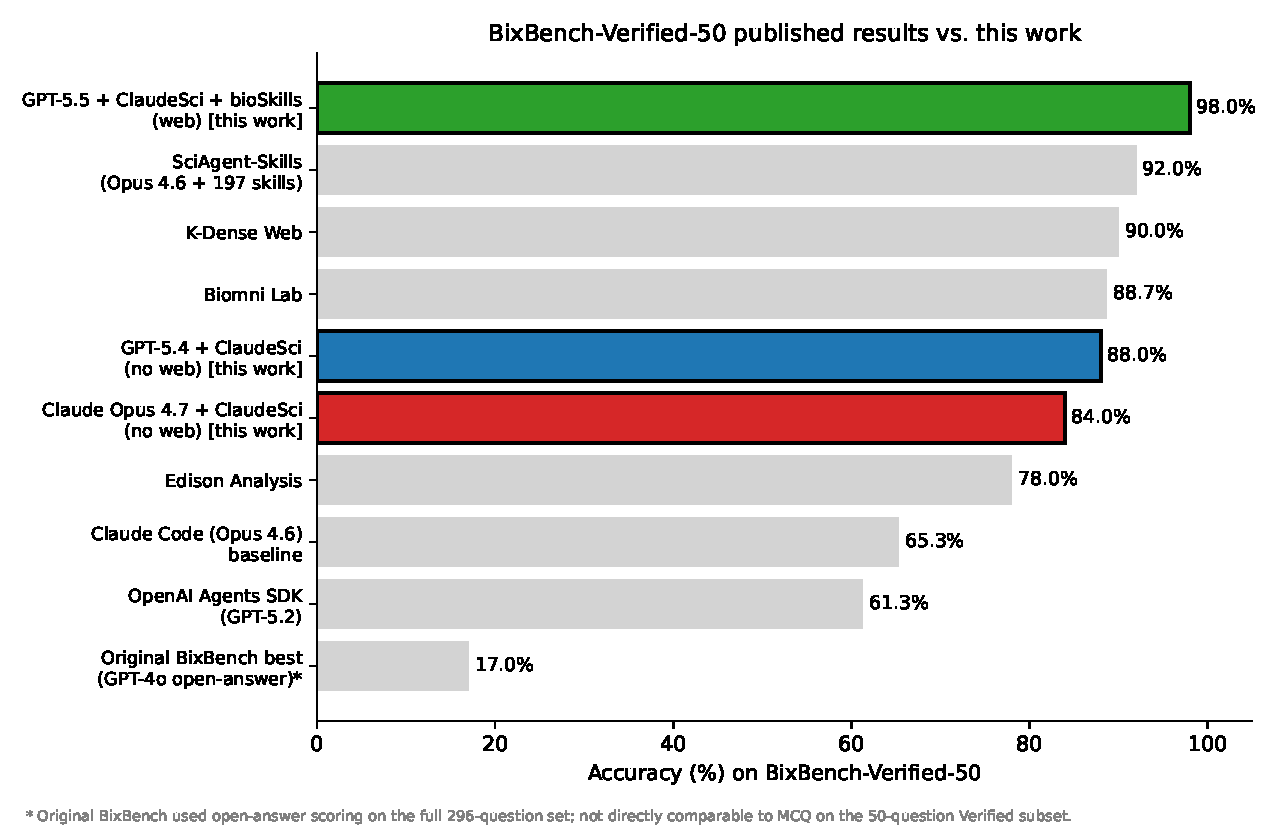
\includegraphics[width=0.95\linewidth]{fig2_leaderboard.pdf}
  \caption{Reported accuracy on BixBench-Verified-50 across published
  agents and the three configurations evaluated in this work
  (highlighted). Numbers for prior systems were taken from the Phylo
  blog \citep{phylo2026}, the K-Dense Web blog \citep{kdense2026}, and
  the SciAgent-Skills repository \citep{sciagent2026}. The original
  BixBench frontier-model number is shown for context but used a
  different scoring protocol on the full 296-question set.}
  \label{fig:leaderboard}
\end{figure}

\subsection{Per-capsule and per-category breakdown}

Figure~\ref{fig:heatmap} shows per-capsule accuracy for all three
configurations. 24 of 32 capsules are answered perfectly by all three
agents (3 in green for every column). Difficulty concentrates in eight
capsules, almost all of which are KEGG/pathway-enrichment problems
(\texttt{bix-26}, \texttt{bix-32}, \texttt{bix-53}), phylogenetics
problems requiring PhyKIT or BUSCO HMM databases (\texttt{bix-11},
\texttt{bix-12}, \texttt{bix-34}, \texttt{bix-38}), or
expression/essentiality questions (\texttt{bix-16}). The web-enabled
configuration recovers all but one of these (\texttt{bix-16}, discussed
below).

\begin{figure}[ht]
  \centering
  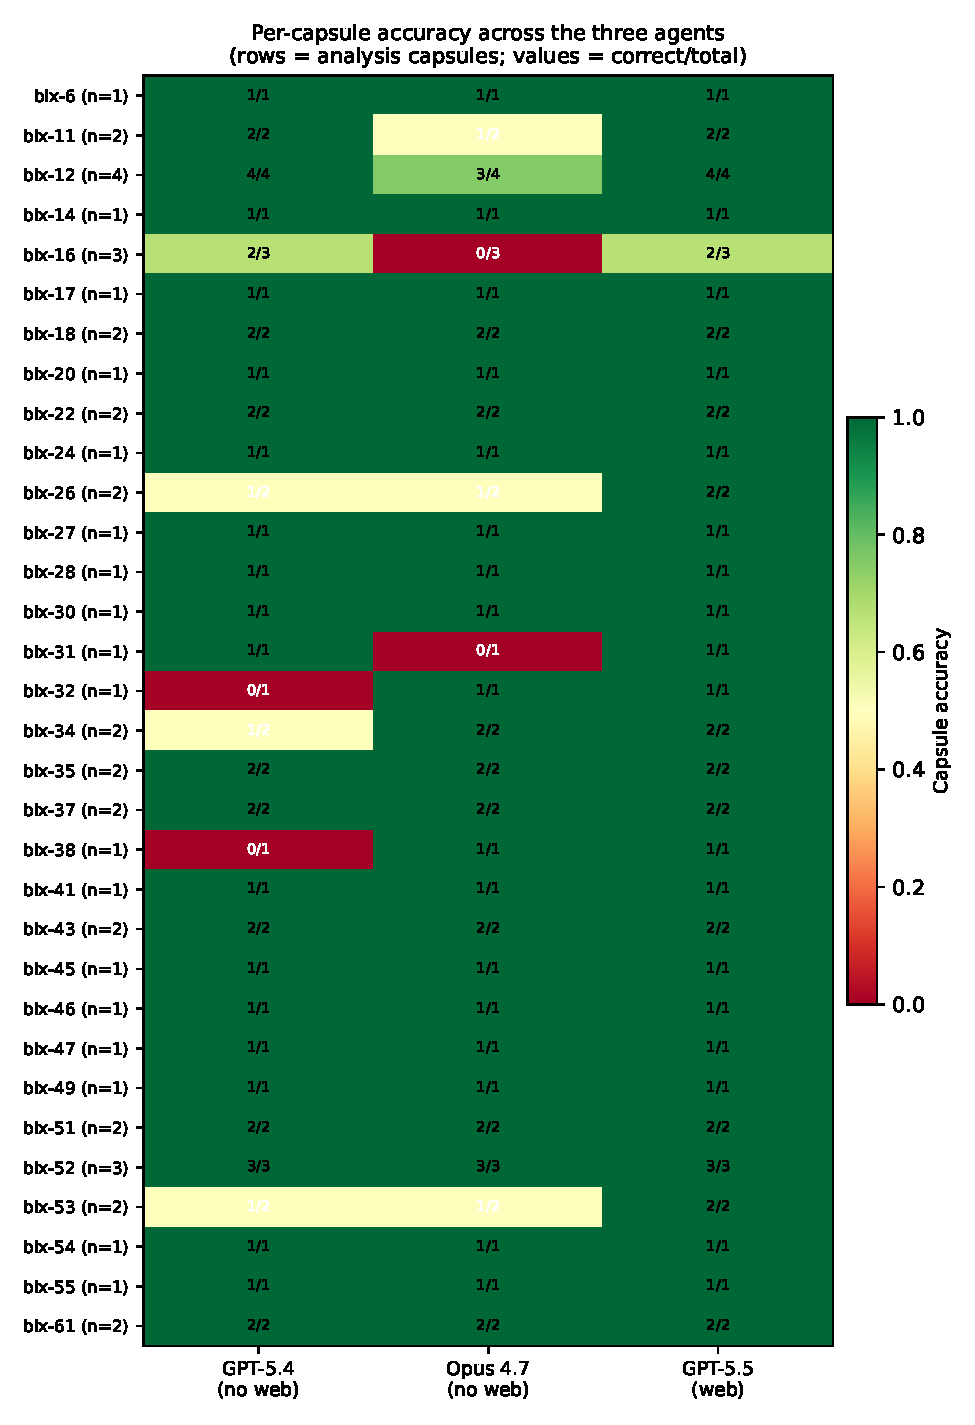
\includegraphics[height=0.85\textheight]{fig3_capsule_heatmap.pdf}
  \caption{Per-capsule accuracy across the three agents. Green: capsule
  fully solved; red: all questions wrong; yellow: partial. Numbers in
  cells are correct/total questions for that capsule. Most failures
  cluster in capsules requiring external pathway annotations (KEGG,
  WikiPathways) or BUSCO/phylogenetics resources.}
  \label{fig:heatmap}
\end{figure}

Figure~\ref{fig:categories} aggregates the same data into eight question
categories. The web-enabled configuration is at 100\% in every category
except CRISPR/essentiality, where the residual error is the
\texttt{bix-16-q1} failure shared by all three agents. The largest gain
from web access + bioSkills appears in the differential-expression /
pathway-enrichment family (12 questions), where it converts a 75\%
score (offline) into 100\%. Phylogenetics/comparative-genomics is the
second-largest beneficiary, recovering the BUSCO-HMM and PhyKIT
failures that the offline agents could not resolve from the local
capsule alone.

\begin{figure}[ht]
  \centering
  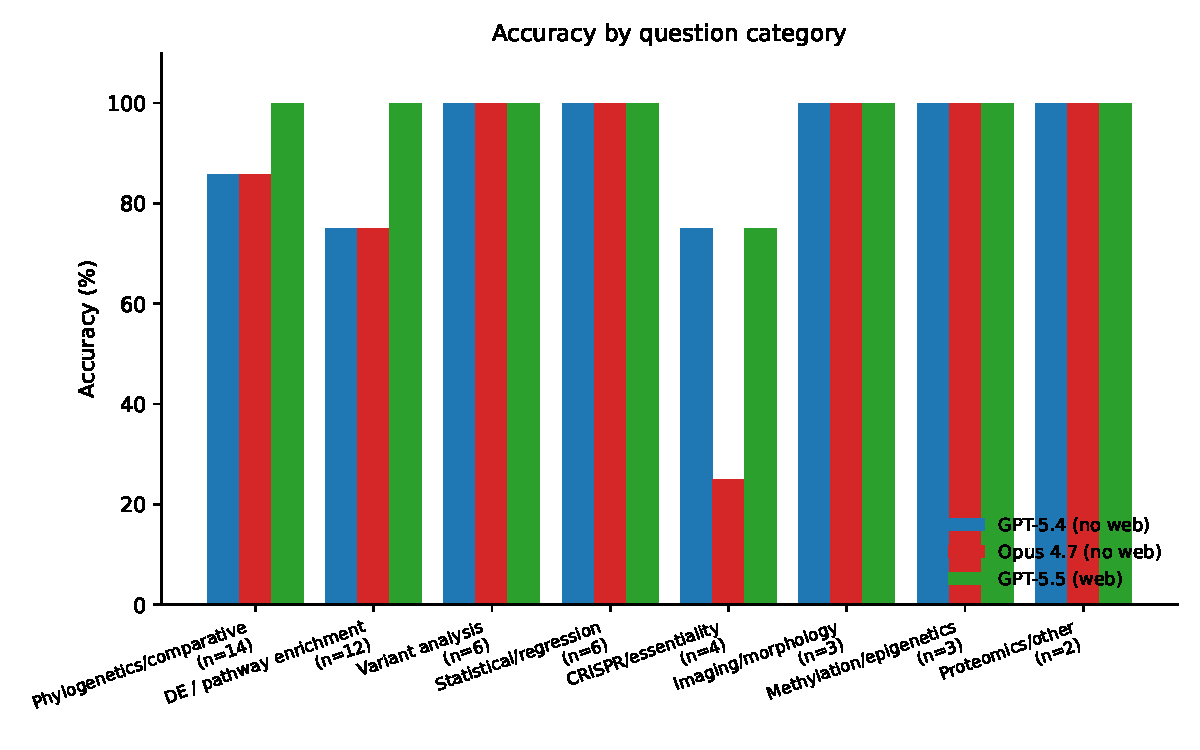
\includegraphics[width=0.95\linewidth]{fig5_categories.pdf}
  \caption{Accuracy by question category (capsules grouped by primary
  analytical task). Web-enabled GPT-5.5 reaches 100\% in every category
  except CRISPR/essentiality, where the single residual error is shared
  by all three agents.}
  \label{fig:categories}
\end{figure}

\subsection{Agreement and shared errors}

The three agents disagree primarily through the offline pair making
different mistakes (Figure~\ref{fig:venn}). Pairwise agreement on
correctness is 76\% between the two offline agents (GPT-5.4 vs.\
Opus~4.7), 90\% between GPT-5.4 (no web) and GPT-5.5 (web), and 86\%
between Opus~4.7 (no web) and GPT-5.5 (web). Strikingly, only one
question (\texttt{bix-16-q1}) is missed by all three agents.

\begin{figure}[ht]
  \centering
  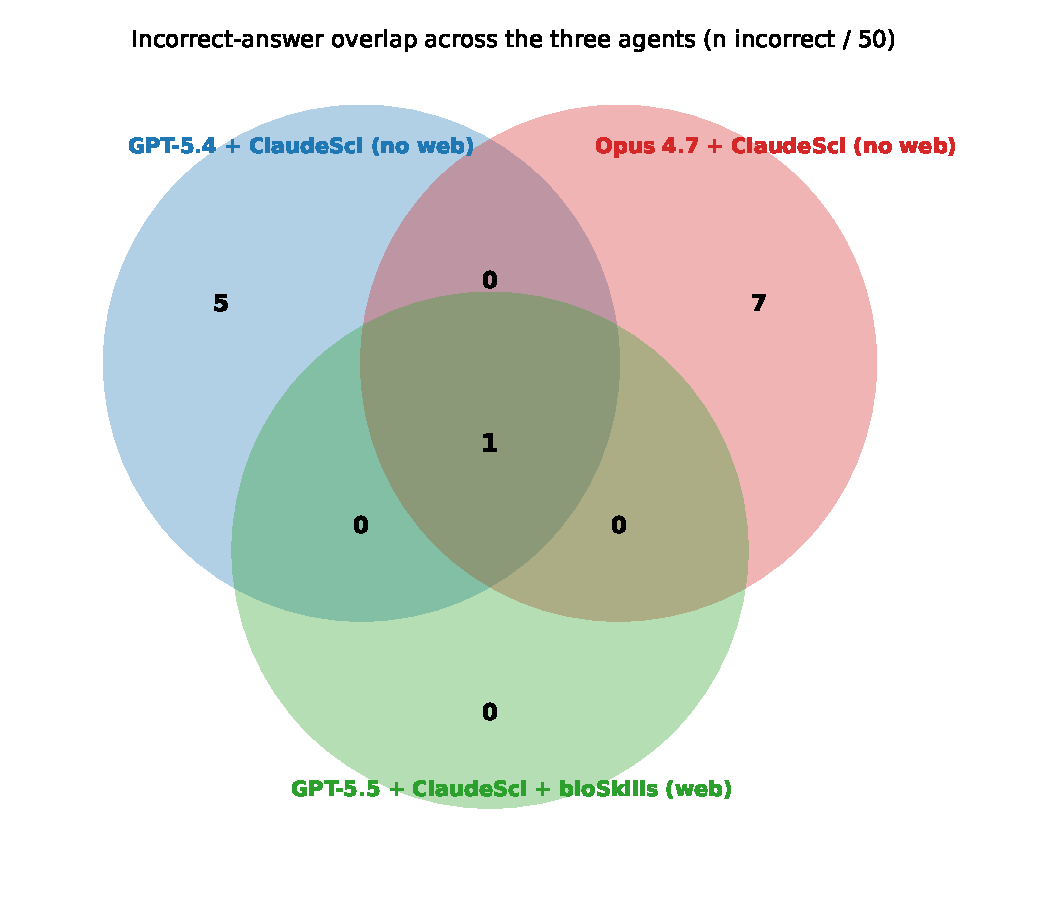
\includegraphics[width=0.7\linewidth]{fig4_venn.pdf}
  \caption{Set diagram of incorrect-answer overlap. The two offline
  configurations make 5 (GPT-5.4) and 7 (Opus~4.7) errors that are
  unique to one of them; only one question is missed by all three
  configurations.}
  \label{fig:venn}
\end{figure}

\subsection{Qualitative error analysis}

We examined every incorrect answer in detail. Errors fall into three
categories.

\paragraph{(i) Missing offline annotations.} The clearest pattern in the
offline configurations is failure on questions that require external
annotation databases the agent does not have locally. GPT-5.4 (no web)
explicitly notes this in its agent summaries:
``\emph{KEGG.db and PA14 OrgDb packages are not installed, and
\texttt{clusterProfiler::enrichKEGG} fails offline when trying to fetch
\texttt{pau} pathway mappings}'' (\texttt{bix-26-q3});
``\emph{the capsule only contains three DESeq2 result files and no KEGG
pathway mapping}'' (\texttt{bix-32-q2});
``\emph{no installed gseapy, no local WikiPathways\_2019\_Mouse library,
and no local mouse annotation package to map the Ensembl mouse gene IDs
to pathway-library gene symbols}'' (\texttt{bix-53-q5}). In each of these
cases the web-enabled GPT-5.5 successfully fetches the necessary library
or annotation and answers correctly. Two phylogenetics questions
(\texttt{bix-38-q1}, \texttt{bix-34-q2}) fail in the offline GPT-5.4
configuration with similar root cause (no installed PhyKIT, no BUSCO
HMM database for the requested gene).

\paragraph{(ii) Off-by-one numerical disagreement.} Several offline
errors involve small numerical disagreements with the gold answer, often
within a factor of 2 of the correct value. The Opus~4.7 errors on
\texttt{bix-31-q2} (FAM138A log$_2$FC) and \texttt{bix-12-q6}
(Mann--Whitney $U$ statistic) are of this flavor; the chosen distractor
is plausible but reflects a different shrinkage method or a different
preprocessing step than the gold notebook used.

\paragraph{(iii) Persistent shared error: \texttt{bix-16-q1}.} The
question asks for the gene with the strongest negative Spearman
correlation between expression and essentiality. All three agents used the
same basic formulation: align expression and \texttt{CRISPRGeneEffect.csv}
by shared cell-line model, compute gene-wise Spearman correlations, and
select the most negative coefficient. Under the raw sign convention in the
distributed CRISPR gene-effect file, this procedure yields CCND1
($\rho=-0.629$), with KLF5 at $\rho=-0.602$ in the GPT-5.5 run. The
reference answer is CDKN1A. Reversing the sign of the gene-effect scores
before correlation changes which direction corresponds to increasing
essentiality and is consistent with the reference answer. We therefore
count \texttt{bix-16-q1} as an official benchmark miss, but interpret it
as a question-wording and sign-convention ambiguity rather than evidence
that the agent failed to perform the requested statistical analysis.

\begin{table}[ht]
\centering
\caption{Incorrect-answer summary. The web-enabled GPT-5.5 configuration
has one official miss, \texttt{bix-16-q1}; review of the trajectory showed
that the computation was correct for the raw \texttt{CRISPRGeneEffect.csv}
sign convention, while the reference answer depends on interpreting
essentiality with the opposite sign.}
\label{tab:errors}
\begin{tabular}{lccp{0.48\linewidth}}
\toprule
Configuration & Official errors & Accuracy & Dominant error mode \\
\midrule
GPT-5.4 (no web) & 6 & 88.0\% &
Missing offline pathway or phylogenetics resources, plus the shared
essentiality sign-convention question. \\
Opus 4.7 (no web) & 8 & 84.0\% &
Mixture of numerical/preprocessing disagreements, pathway analysis errors,
and the shared essentiality sign-convention question. \\
GPT-5.5 (web) & 1 & 98.0\% &
Only \texttt{bix-16-q1}; no clear computational failure after trajectory
review. \\
\bottomrule
\end{tabular}
\end{table}

\section{Discussion}\label{sec:discussion}

\subsection{Are SOTA agents ready for bioinformatics?}

The headline answer from this work is that, for the kind of short,
well-specified analytical question represented in BixBench-Verified-50,
frontier agents with appropriate scientific skills are now within one
question of perfect performance. The single remaining GPT-5.5 miss appears
to be a sign-convention ambiguity rather than a failure to load, clean,
analyze, or statistically interpret the data. This is a substantial shift
from the picture in the original BixBench paper a year ago, and it calls
for a narrower conclusion than either optimism or skepticism alone would
support: these agents are already highly capable on bounded,
well-specified bioinformatics tasks, but that does not mean they can yet
replace expert oversight on open-ended research projects.

The 88\%-then-98\% pattern across our two GPT configurations is
particularly informative because the no-web GPT-5.4 configuration already
performs in the same range as previously reported leading systems. This
suggests that a competent base model plus a curated scientific-skill
library is sufficient for many routine benchmark tasks where the required
data are local and the expected analysis is well defined. Web access
changes the picture mainly by filling gaps in offline annotation
databases and software packages (KEGG, WikiPathways, PhyKIT, BUSCO HMM
models, mouse OrgDb), a narrow but common class of problems in practical
bioinformatics.

\subsection{Where the easy gains came from}

Our category-level breakdown (Figure~\ref{fig:categories}) makes the
locus of improvement explicit. Variant analysis, statistical/regression,
imaging/morphology, methylation, and proteomics are at 100\% for all
three configurations: these are tasks where everything the agent needs
is in the capsule. Phylogenetics and DE/pathway-enrichment are the
categories where web access matters, because both rely on external
annotation resources or specialized software (PhyKIT, BUSCO,
clusterProfiler, gseapy with Mouse pathway libraries). Within these
two categories, the ``hard'' questions are uniformly resolved by GPT-5.5
(web) once the agent can install the required package or fetch the
required pathway file. This is consistent with the SciAgent-Skills
report \citep{sciagent2026}, which observed a +26.7-point lift on
BixBench-Verified-50 simply by equipping Claude Code (Opus~4.6) with
197 bioinformatics skills, no fine-tuning required.

\subsection{Limitations of BixBench-Verified-50 as an
``agent readiness'' test}

While BixBench-Verified-50 is the cleanest publicly available agent
benchmark for bioinformatics, it has structural features that make it
easier than typical research analysis. (a) Questions are
multiple-choice with at most five options; the prior on a random guess
is 25\% rather than effectively zero for an open answer. (b) Each
question is associated with one curated capsule that contains the
relevant input data; the agent does not have to discover the data or
determine its provenance. (c) The questions are derived from published,
peer-reviewed analytical workflows, so a correct procedure provably
exists; this is not the situation in exploratory analysis. (d) The
``Insufficient information'' refusal option is itself a hint to a
calibrated agent that the question is answerable. (e) The 50 questions
are short --- typically under a few hundred LOC of code on the agent
side --- whereas a real dissertation chapter analysis might be tens of
thousands of lines.

The mismatch between BixBench-style questions and the real day-to-day
work of a computational biologist is the central caveat to our
conclusion. Phylo's recent BiomniBench framework \citep{phylo2026}
attempts to address this by scoring agents on the entire analytical
trace rather than just the final number; we view that direction as
strictly complementary to the work here. Saturating BixBench-Verified-50
is necessary but probably not sufficient for ``agent readiness''.

\subsection{Implications for skill libraries}

Our results suggest that the most cost-effective way to upgrade a
generic frontier-model coding agent for bioinformatics is to attach a
curated skill library, not to build a bespoke multi-agent architecture.
The comparison is not a perfect ablation, because model versions differ
across public leaderboard entries, but the pattern is consistent across
our runs and external reports: agents with explicit scientific skills
perform far better than vanilla coding-agent baselines on the same
verified benchmark \citep{phylo2026,kdense2026,sciagent2026}. Stacking a
second skill library (bioSkills) plus web access on top of a stronger base
model yields the highest score we have seen reported. Skill libraries also
have the appealing property that they are inspectable, version-controlled
markdown \citep{anthropicskills}, and therefore reviewable by domain
experts in a way that a fine-tuned weights-only model is not.

\subsection{What's still missing}

Three things would change our headline conclusion. First, we did not
evaluate end-to-end \emph{open-answer} performance on these capsules; the
original BixBench numbers were dramatically lower in open-answer mode,
and skill libraries may not close that gap as completely as they close
the MCQ gap. Second, we did not measure trace quality: a 98\% accuracy
agent that arrives at correct answers via incorrect intermediate steps
would still mislead a human collaborator. Third, the questions in
BixBench-Verified-50 are designed around 1--3 day analyses; nothing in
this benchmark validates that an agent can autonomously sustain
multi-week analytical projects with shifting hypotheses, which is
arguably what real ``agent readiness'' for biology research would
require.

\section{Conclusion}

Frontier-model agents equipped with curated scientific skills are
markedly more capable on bioinformatics tasks than they were a year ago.
On BixBench-Verified-50 our offline configurations (84\% and 88\%)
already match the previously reported leaderboard band, and our
web-enabled GPT-5.5 + Claude Scientific Skills + bioSkills configuration
sets a new high (98\%, 49/50), with only one official miss and no clear
computational failure after trajectory review. The locus of improvement is
concentrated in tasks that require external annotation databases or
specialized software: web access is not magic, it is a targeted fix for
offline gaps. Skill libraries are an unusually cost-effective lever,
contributing substantial headline accuracy while remaining inspectable by
domain experts. We caution that BixBench-Verified-50 measures a
particular, narrow slice of bioinformatics research; near-saturation is
necessary but not sufficient evidence that frontier agents can replace
experienced computational biologists. Trace-level evaluations
\citep{phylo2026,huang2025biomni}, open-answer benchmarks, and longer
analytical projects are the natural next tests.

\section*{Data and Code Availability}
Per-agent prediction CSVs (\texttt{combined.csv}), grading JSONs
(\texttt{combined\_graded.json}), grading reports
(\texttt{combined\_grading\_report.md}), per-question correctness
matrix (\texttt{per\_question\_correctness.csv}), figure-generation code
(\texttt{make\_figures.py}), and per-capsule analysis script
(\texttt{agent\_results.py}) are bundled with this manuscript.
BixBench-Verified-50 is available at
\url{https://huggingface.co/datasets/phylobio/BixBench-Verified-50}.

\section*{Acknowledgments}
We thank the FutureHouse and ScienceMachine teams for releasing
BixBench, the Phylo team for curating BixBench-Verified-50, and the
maintainers of Claude Scientific Skills (K-Dense AI) and bioSkills
(GPTomics) for releasing their skill libraries under permissive
licences.

\section*{Competing Interests}
The author declares no competing interests.

\bibliographystyle{unsrtnat}
\bibliography{references}

\end{document}
